\chapter{Types}
\label{ch:types}
This Section defines Type Literals using EBNF and RegEx.
\section{Generic Types}
\label{sec:generic-types}
\subsection{Boolean}
\subsubsection{Boolean Data Type Definition}
The Boolean data type represents logical truth values. It has exactly two possible values: \texttt{True} and \texttt{False}. Booleans are used in conditional expressions, logical operations, and control flow decisions.

\subsubsection{Boolean Data Type Literals}
\begin{verbatim}
boolean_literal = "True" | "False"
\end{verbatim}
\subsubsection{Boolean Data Type Casting and Coercion}
Boolean values can be coerced from other types:
\begin{itemize}
\item Int and real values coerce to \texttt{False} if zero, \texttt{True} otherwise
\item Strings coerce to \texttt{False} if empty, \texttt{True} otherwise
\item Lists and Sets coerce to \texttt{False} if empty, \texttt{True} otherwise
\item \texttt{None} coerces to \texttt{False}
\end{itemize}
Explicit conversion is not supported; boolean evaluation is implicit in conditional contexts.
\subsection{Integer}
\subsubsection{Integer Data Type Definition}
The Integer data type represents whole numbers (elements of $\mathbb{Z}$). Integers support standard arithmetic operations and can express values from very large negative to very large positive using SI decimal prefixes (kilo and above).
\subsubsection{Integer Data Type Literals}
Integer literals can be expressed in multiple formats:
\begin{verbatim}
EBNF:
int_literal = decimal_int | binary_literal 
            | octal_literal | hex_literal

decimal_int = ["+" | "-"], digit, {digit}

binary_literal   = "0b", bindigit, {bindigit}
octal_literal    = "0o", octdigit, {octdigit}
hex_literal      = "0x", hexdigit, {hexdigit}

RegEx:
digit     = [0-9]
bindigit  = [01]
octdigit  = [0-7]
hexdigit  = [0-9a-fA-F]
\end{verbatim}

SI prefixes >= k produce integers:
\begin{verbatim}
6.2k    #c# = 6200 (int)
1M      #c# = 1000000 (int)
-5e9    #c# = -5000000000 (int)
4Q      #c# = 4e30 (int)
\end{verbatim}

Binary, octal, and hex literals always produce integers:
\begin{verbatim}
0x10    #c# = 16
0b1010  #c# = 10
0o17    #c# = 15
\end{verbatim}

\subsubsection{Integer Data Type Casting and Coercion}
Integers can be coerced from other types:
\begin{itemize}
\item Booleans coerce to \texttt{0} (False) or \texttt{1} (True)
\item Numeric strings with no decimal point are parsed as integers (e.g., \texttt{"42"} becomes \texttt{42})
\item \texttt{real} values are truncated (e.g., \texttt{int(3.7)} becomes \texttt{3})
\end{itemize}

\subsection{Real}
\subsubsection{Real Data Type Definition}
The Real data type represents floating-point numbers (elements of $\mathbb{R}$). Reals support standard arithmetic operations and can express values from very small (quecto-scale, $10^{-30}$) to very large (quetta-scale, $10^{30}$) using SI decimal prefixes.
\subsubsection{Real Data Type Literals}
Real literals can be expressed in multiple formats:
\begin{verbatim}
EBNF:
real_literal = decimal_real | scientific_real

decimal_real   = ["+" | "-"], digit, {digit}, ".", {digit}
               | ["+" | "-"], ".", digit, {digit}

scientific_real = ["+" | "-"], digit, {digit}, 
                  ["." , {digit}], ("e" | "E"), 
                  ["+" | "-"], digit, {digit}
\end{verbatim}

A literal with a decimal point or scientific notation produces a real, even if the fractional part is zero:
\begin{verbatim}
3.14    #c# = 3.14 (real)
42.0    #c# = 42.0 (real)
42e0    #c# = 42.0 (real)
.4      #c# = 0.4 (real)
2e-6    #c# = 0.000002 (real)
\end{verbatim}

SI prefixes below k produce reals:
\begin{verbatim}
100n    #c# = 0.0000001 (real)
1m      #c# = 0.001 (real)
5c      #c# = 0.05 (real)
\end{verbatim}

The full SI prefix table:
\begin{verbatim}
SI_Prefixes:
q  1e-30  quecto     Q  1e+30  quetta
r  1e-27  ronto      R  1e+27  ronna
y  1e-24  yocto      Y  1e+24  yotta
z  1e-21  zepto      Z  1e+21  zetta
a  1e-18  atto       E  1e+18  exa
f  1e-15  femto      P  1e+15  peta
p  1e-12  pico       T  1e+12  tera
n  1e-9   nano       G  1e+9   giga
u  1e-6   micro      M  1e+6   mega
m  1e-3   milli      k  1e+3   kilo
c  1e-2   centi
d  1e-1   deci
\end{verbatim}

Prefixes >= k produce integers. Prefixes < k produce reals.

\subsubsection{Real Data Type Casting and Coercion}
Reals can be coerced from other types:
\begin{itemize}
\item Integers coerce to real (e.g., \texttt{real(5)} becomes \texttt{5.0})
\item Booleans coerce to \texttt{0.0} (False) or \texttt{1.0} (True)
\item Numeric strings with a decimal point are parsed as reals (e.g., \texttt{"3.14"} becomes \texttt{3.14})
\item Non-numeric strings raise a type error
\end{itemize}
Lists of ints or reals can be passed to mathematical functions, which operate element-wise.
\subsection{Complex}
\subsubsection{Complex Data Type Definition}
The Complex data type represents complex numbers (elements of $\mathbb{C}$). A complex number has a real part and an imaginary part, and can be expressed in rectangular or polar form.

\paragraph{Type Hierarchy}
\begin{center}
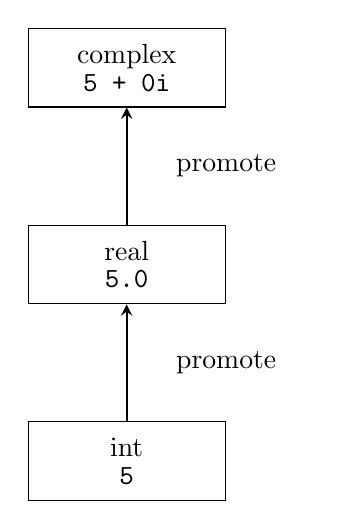
\begin{tikzpicture}[>=stealth, node distance=2.5cm, every node/.style={draw, rectangle, minimum width=2.5cm, minimum height=1cm, align=center}]
  \node (complex) {complex\\[-2pt]\texttt{5 + 0i}};
  \node (real) [below of=complex] {real\\[-2pt]\texttt{5.0}};
  \node (int) [below of=real] {int\\[-2pt]\texttt{5}};
  \draw[->, thick] (int) -- node[right, draw=none] {promote} (real);
  \draw[->, thick] (real) -- node[right, draw=none] {promote} (complex);
\end{tikzpicture}
\end{center}

Auto-promotion is implicit and lossless: an \texttt{int} can be used wherever a \texttt{real} is expected, and both can be used wherever a \texttt{complex} is expected.

\subsubsection{Complex Data Type Literals}
\begin{verbatim}
EBNF:
complex_literal = rectangular_literal | polar_literal

rectangular_literal = ["+" | "-"], number, ["+", number, "i"] 
                    | ["+" | "-"], number, "-", number, "i"
                    | ["+" | "-"], number, "i"

polar_literal = number, "<|", number
\end{verbatim}

The \texttt{i} suffix on a number creates a complex literal. The \texttt{<|} operator creates a polar literal (magnitude <| angle in radians).

\paragraph{Rectangular Form}
\begin{verbatim}
3 + 4i        #c# real=3, imag=4
-2 - 7i       #c# real=-2, imag=-7
5i            #c# real=0, imag=5
3             #c# real=3, imag=0 (int promoted to complex)
3.14 + 2.71i  #c# real=3.14, imag=2.71
\end{verbatim}

Note: \texttt{3 + 4i} is parsed as \texttt{3 + (4i)} -- the \texttt{+} is the addition operator, and \texttt{4i} is a single complex literal. This means complex arithmetic uses the same operators as other numeric types.

\paragraph{Polar Form}
\begin{verbatim}
2 <| 1.5708    #c# magnitude=2, angle=pi/2 (radians)
1 <| 0         #c# magnitude=1, angle=0 (real number 1)
1 <| 3.14159   #c# magnitude=1, angle=pi (real number -1)
\end{verbatim}

\subsubsection{Complex Data Type Casting and Coercion}
\begin{itemize}
\item \texttt{int} promotes to \texttt{complex}: \texttt{5} becomes \texttt{5 + 0i}
\item \texttt{real} promotes to \texttt{complex}: \texttt{3.14} becomes \texttt{3.14 + 0i}
\item Mixed operations (\texttt{int + complex}, \texttt{real + complex}) produce \texttt{complex}
\item \texttt{complex} cannot be coerced to \texttt{real} or \texttt{int} (use \texttt{real()} or \texttt{int()} to extract parts)
\item Booleans coerce to \texttt{complex}: \texttt{True} becomes \texttt{1 + 0i}
\item Lists of complex can be passed to mathematical functions, which operate element-wise
\end{itemize}

\subsubsection{Complex Components}
The real and imaginary parts of a complex number are accessed via functions:
\begin{verbatim}
real($z)   #c# Returns the real part (real)
imag($z)   #c# Returns the imaginary part (real)
\end{verbatim}
See Section~\ref{sec:complex_functions} for full documentation.
\subsection{Set}
\subsubsection{Set Data Type Definition}
A Set is an unordered collection of unique elements. Sets can contain any data type:
\begin{itemize}
\item Integers and reals (numbers)
\item Strings
\item Booleans
\item Lists
\item Parts
\item Connections
\item Pins
\item Nets
\end{itemize}

Sets containing mixed types are allowed. Duplicate elements are automatically removed. Sets support standard set algebra operations (union, intersection, difference, subset, element-of).

\subsubsection{Set Data Type Literals}
\begin{verbatim}
EBNF:
set_literal = "{", [ { data, ","}, data ], "}"
\end{verbatim}

Examples:
\begin{verbatim}
$numbers [set]= { 1, 2, 3, 4, 5 }
$mixed [set]= { 1, "hello", True, Q1 }
$parts [set]= { Q1, Q2, R3 }
\end{verbatim}

Sets also support range generation using the same syntax as lists:
\begin{verbatim}
{start:increment:end}    #c# explicit increment
{start:end}              #c# increment defaults to 1
{start|end|count}        #c# evenly spaced, count elements
\end{verbatim}
Examples:
\begin{verbatim}
$evens [set]= {0:2:10}      #c# {0, 2, 4, 6, 8, 10}
$range [set]= {0:5}         #c# {0, 1, 2, 3, 4, 5}
$lin   [set]= {0|1|5}       #c# {0, 0.25, 0.5, 0.75, 1}
\end{verbatim}

Note: since sets are unordered and unique, duplicates within a range are silently ignored. For example, \texttt{\{0:0.3:1\}} produces \texttt{\{0, 0.3, 0.6, 0.9\}} with no duplicate \texttt{0} entries.

\subsubsection{Set Data Type Casting and Coercion}
Sets can be created from Lists using the \texttt{f.set()} function. When converting a List to a Set, duplicate elements are removed and order is lost.\\
Example:
\begin{verbatim}
$my_list [list]= [ 1, 2, 2, 3, 3, 3 ]
$my_set [set]= f.set( $my_list )  #c# { 1, 2, 3 }
\end{verbatim}
Sets can be converted to Lists using the \texttt{f.list()} function. The order of elements in the resulting List is determined by the order they appear in the global set \texttt{*e}.
\subsection{String}
\subsubsection{String Data Type Definition}
The String data type represents textual data. Strings can be delimited by single or double quotes, and support escape sequences. Long strings (multi-line) are delimited by triple quotes.
\subsubsection{String Data Type Literals}
\begin{verbatim}
EBNF:
string_literal = long_string | short_string
short_string   =   '"', {short_string_item_I},  '"'   |
                   "'", {short_string_item_II}, "'"
long_string    = '"""',  {long_string_item_I},  '"""' |
                 "'''",  {long_string_item_II}, "'''"

RegEx:
short_string_item_I  = [^"\\\n)]|(\\.)
short_string_item_II = [^'\\\n)]|(\\.)
 long_string_item_I  = [^"\\]|(\\.)
 long_string_item_II = [^'\\]|(\\.)
\end{verbatim}
\subsubsection{String Data Type Casting and Coercion}
Strings can be created from other types using the \texttt{f.str()} function, which concatenates all arguments into a single string.\\
Example:
\begin{verbatim}
$msg [string]= f.str( "The value is ", 42, 
    " and color is ", "red" )
#c# $msg = "The value is 42 and color is red"
\end{verbatim}
Additional string functions include \texttt{f.upperc()} (uppercase), \texttt{f.lowerc()} (lowercase), and \texttt{f.format()} (formatted output).
\subsection{List}
\subsubsection{List Data Type Definition}
The List data type represents an ordered, indexed collection of objects. Lists support 0-based indexing, slicing, and can contain elements of different types. Lists are mutable and can be dynamically resized.
\subsubsection{List Data Type Literals}
\begin{verbatim}
EBNF:
list_literal = "[", [{ data, "," }, data], "]"
\end{verbatim}
\subsubsection{List Data Type Casting and Coercion}
Lists can be created from Sets using the \texttt{f.list()} function. The order is determined by the element order in \texttt{*e}.\\
Lists support range generation using the syntax:
\begin{verbatim}
[start:increment:end]    #c# explicit increment
[start:end]              #c# increment defaults to 1
[start|end|count]        #c# evenly spaced, count elements
\end{verbatim}
Examples:
\begin{verbatim}
$r1 [list]= [0:2:10]      #c# [0, 2, 4, 6, 8, 10]
$r2 [list]= [0:5]         #c# [0, 1, 2, 3, 4, 5]
$r3 [list]= [0|1|5]       #c# [0, 0.25, 0.5, 0.75, 1]
\end{verbatim}
\subsubsection{Ndarray (N-dimensional Array)}
An ndarray is a list that is \textbf{rectangular} (all sublists have the same length) and contains only \textbf{numeric} values (\texttt{int} or \texttt{real}). Ndarray status is determined automatically -- no type annotation is needed. A list that is rectangular and all-numeric gains ndarray operations; all other lists remain standard lists.

\paragraph{Detection Rules}
\begin{itemize}
\item A list is an ndarray if all elements are \texttt{int} or \texttt{real}, and all sublists (if any) have identical length.
\item Nested lists of different lengths are NOT ndarrays: \texttt{[[1,2], [3,4,5]]} is a standard list.
\item Lists containing strings, bools, or other non-numeric types are NOT ndarrays.
\item Empty lists \texttt{[]} and flat numeric lists \texttt{[1, 2, 3]} are ndarrays (1D).
\end{itemize}

\paragraph{Shape}
The shape of an ndarray is described by its dimensions:
\begin{itemize}
\item 1D: \texttt{[1, 2, 3]} has shape \texttt{(3)}
\item 2D: \texttt{[[1,2], [3,4], [5,6]]} has shape \texttt{(3, 2)} (3 rows, 2 columns)
\end{itemize}

\paragraph{Broadcasting}
When an ndarray is combined with a scalar, the scalar is broadcast to match the ndarray's shape:
\begin{verbatim}
[1, 2, 3] + 5          #c# = [6, 7, 8]
[1, 2, 3] * 2          #c# = [2, 4, 6]
[[1,2],[3,4]] + 10      #c# = [[11,12],[13,14]]
\end{verbatim}

\paragraph{Element-wise Operations}
When two ndarrays of the same shape are combined with a standard operator (\texttt{+}, \texttt{-}, \texttt{*}, \texttt{/}, \texttt{\%}, \texttt{\^{}}), the operation is applied element-wise:
\begin{verbatim}
[1, 2, 3] + [4, 5, 6]     #c# = [5, 7, 9]
[1, 2, 3] * [4, 5, 6]     #c# = [4, 10, 18]
[10, 20, 30] - [1, 2, 3]  #c# = [9, 18, 27]
[10, 20, 30] / [2, 4, 5]  #c# = [5.0, 5.0, 6.0]
\end{verbatim}

\paragraph{Slicing}
Ndarrays (and all lists) support Python-style slicing with the syntax \texttt{list[start:stop:step]}:
\begin{itemize}
\item \texttt{list[start:stop]} -- elements from \texttt{start} up to (not including) \texttt{stop}
\item \texttt{list[start:]} -- from \texttt{start} to end
\item \texttt{list[:stop]} -- from beginning to \texttt{stop}
\item \texttt{list[:]} -- full copy
\item \texttt{list[start:stop:step]} -- with step size
\item Negative indices count from the end: \texttt{list[-1]} is the last element
\end{itemize}
\begin{verbatim}
$a [list]= [0, 1, 2, 3, 4, 5]
$a[1:4]       #c# = [1, 2, 3]
$a[2:]        #c# = [2, 3, 4, 5]
$a[:3]        #c# = [0, 1, 2]
$a[::2]       #c# = [0, 2, 4]  (every 2nd element)
$a[-2:]       #c# = [4, 5]     (last 2 elements)
$a[::-1]      #c# = [5, 4, 3, 2, 1, 0]  (reversed)
\end{verbatim}

\paragraph{Reshape}
Ndarrays support reshaping via the \texttt{.reshape()} method. The total number of elements must remain constant.
\begin{verbatim}
$b [list]= [[1,2,3],[4,5,6]]
$b.reshape(3, 2)   #c# = [[1,2],[3,4],[5,6]]
$b.reshape(6)      #c# = [1, 2, 3, 4, 5, 6]  (flatten)
$b.reshape(1, 6)   #c# = [[1,2,3,4,5,6]]     (row vector)
\end{verbatim}

\section{Electrical Types}
\subsection{Part}
\subsubsection{Part Data Type Definition}
A Part represents a physical electronic component in the circuit. Each Part has a reference designator, a model type, a description, and a footprint. Parts contain Pins which can be connected to Nets or other Pins.
\subsubsection{Part Data Type Literals}
Parts are created using the \texttt{elec.part} statement:
\begin{verbatim}
EBNF:
part_statement = "elec.part", part_reference, 
  ":", model_name, "(", [model_params], ")", 
  ";", "des", "=", string_type, 
  ";", "fp", "=", string_type

part_reference = string_type | 
  "[", { string_type, "," }, string_type, "]"
model_name     = id
model_params   = [ { id, "=", data, "," }, 
                   id, "=", data ]
\end{verbatim}
Examples:
\begin{verbatim}
elec.part "R1": r( R = 100, P = 0.25, 
    type = "metal film" )
    ; des = "100 ohm resistor"
    ; fp = "Resistor_SMD:R_0805_2012Metric"

elec.part ["R2", "R3"]: r( R = 220, P = 0.25 )
    ; des = "220 ohm resistors"; fp = "Resistor_SMD:R_0805_2012Metric"
\end{verbatim}
\subsubsection{Part Data Type Casting and Coercion}
Parts cannot be cast from other types. Parts are created via \texttt{elec.part} statements and accessed by their reference designator. Parts support the following properties:
\begin{itemize}
\item Model parameters (accessed via model-specific syntax)
\item Pin references (using \texttt{part\_ref[pin\_ref]} syntax)
\item Description (set via \texttt{des} parameter)
\item Footprint (set via \texttt{fp} parameter)
\end{itemize}
\subsection{Pin}
\subsubsection{Pin Data Type Definition}
A Pin represents a connection point on a Part. Pins are referenced using the syntax \texttt{part\_ref[pin\_ref]}, where \texttt{pin\_ref} is typically a numeric index or a named terminal (e.g., \texttt{R1[1]}, \texttt{Q1[d]}, \texttt{U1[v+]}).
\subsubsection{Pin Data Type Literals}
Pins are created implicitly when Parts are instantiated. Pin references are formed using the bracket notation:
\begin{verbatim}
pin_literal = part_ref, "[", pin_ref, "]"

Examples:
R1[1]      #c# Pin 1 of resistor R1
Q1[d]      #c# Drain pin of MOSFET Q1
U1[v+]     #c# Non-inverting input of op-amp U1
J1[3]      #c# Pin 3 of connector J1
\end{verbatim}
The available pin references depend on the Part's footprint and model definition.
\subsubsection{Pin Data Type Casting and Coercion}
Pins cannot be cast from other types. Pins are accessed via Part references and support the following operations:
\begin{itemize}
\item Connection to other Pins or Nets via \texttt{elec.connect}
\item Membership testing in Sets
\item Iteration over Pins of a Part
\end{itemize}
\subsection{Connection}
\subsubsection{Connection Data Type Definition}
A Connection represents an electrical connection between two Pins. Connections are binary (exactly two Pins) and are created using the pipe syntax or the \texttt{elec.connect} statement.
\subsubsection{Connection Data Type Literals}
Connections can be created using the pipe syntax:
\begin{verbatim}
connection_literal = "(", pin, "|", pin, ")"

Example:
( R2[1] | J4[7] )  #c# R2 pin 1 to J4 pin 7
\end{verbatim}
Connections are also created implicitly by \texttt{elec.connect} statements.
\subsubsection{Connection Data Type Casting and Coercion}
Connections cannot be cast from other types. Connections support:
\begin{itemize}
\item Membership testing in Sets
\item Property queries (length, resistance, inductance, capacitance, impedance)
\end{itemize}
\subsection{Net}
\subsubsection{Net Data Type Definition}
A Net represents a named electrical node that connects multiple Pins and Connections. Nets are the fundamental grouping mechanism in the electrical system, allowing multiple components to share a common electrical connection.
\subsubsection{Net Data Type Literals}
Nets are created using the \texttt{elec.net} statement:
\begin{verbatim}
EBNF:
net_statement = "elec.net", string_type, { string_type }

Example:
elec.net "Gnd"
elec.net "hvbus" "hv" "high_i" "noisy"
\end{verbatim}
The first argument is the net name; subsequent arguments are optional tags.
\subsubsection{Net Data Type Casting and Coercion}
Nets cannot be cast from other types. Nets support:
\begin{itemize}
\item Tagging/untagging via \texttt{elec.tag} and \texttt{elec.untag}
\item Membership testing in Sets
\item Connection to Pins via \texttt{elec.connect}
\item Querying connected objects using quantifier syntax (e.g., \texttt{I@Gnd}, \texttt{P@Vin})
\end{itemize}


\chapter{Variables}
Variables in EDADSL are prefixed with the \texttt{\$} character and are assigned values using type-specific assignment operators.

\section{Variable Declaration and Assignment}
Variables are declared and assigned simultaneously using the following syntax:
\begin{verbatim}
EBNF:
variable            = "$", id
variable_assignment = variable, (typed_assign | inferred_assign),
                      [",", "M", "=", boolean]

typed_assign        = "[", type, "]", "=", data
inferred_assign     = "t", "=", data

type                = "bool" | "int" | "real" | "list" | "string" 
                    | "set" | "part" | "connection" | "pin" 
                    | "net"
\end{verbatim}

\subsection{Type-Inferred Assignment}
As syntax sugar, \texttt{\$var t= val} is equivalent to \texttt{\$var [type(val)]= val}. The type is inferred from the value at assignment time.
\begin{verbatim}
$a t= 3              #c# Equivalent to $a [int]= 3
$name t= "EDADSL"    #c# Equivalent to $name [string]= "EDADSL"
$flag t= True        #c# Equivalent to $flag [bool]= True
$colors t= [1, 2, 3] #c# Equivalent to $colors [list]= [1, 2, 3]
\end{verbatim}

The type determines the variable's data type:
\begin{itemize}
\item \texttt{bool} -- Boolean
\item \texttt{int} -- Integer
\item \texttt{real} -- Real
\item \texttt{complex} -- Complex number
\item \texttt{list} -- List
\item \texttt{string} -- String
\item \texttt{set} -- Set
\item \texttt{part} -- Part
\item \texttt{connection} -- Connection
\item \texttt{pin} -- Pin
\item \texttt{net} -- Net
\end{itemize}

\section{Mutability}
By default, variables are mutable (can be reassigned). To make a variable immutable, append \texttt{; M = False} after the assignment:
\begin{verbatim}
$immutable [int]= 42; M = False
$mutable [int]= 100    #c# Can be reassigned
\end{verbatim}

\section{Scope}
Variables have global scope once declared. They can be accessed from any point in the program after their declaration. There is no block scoping for \texttt{if} or \texttt{for} blocks; variables declared inside these remain accessible outside. However, variables declared inside functions are local to that function and shadow any global variables of the same name (see Section~\ref{sec:function-scope}).

\section{Examples}
\begin{verbatim}
$a [int]= 3
$b [int]= 5
$result [int]= $a + $b        #c# Scalar assignment

$name [string]= "EDADSL"         #c# String assignment
$flag [bool]= True               #c# Boolean assignment

$colors [list]= ["red", "green", "blue"]  #c# List
$hwset [set]= { Q1, Q2, R5 }              #c# Set
\end{verbatim}


\chapter{Expressions}
Expressions in EDADSL evaluate to values and can be composed of literals, variables, function calls, and operators.

\section{Expression Grammar}
\begin{verbatim}
EBNF:
expression          = arithmetic_expression
                    | boolean_expression
                    | comparison_expression
                    | set_expression
                    | postfix_expression
                    | function_call
                    | lambda
                    | "(" expression ")"

arithmetic_expression = expression,
    ("+" | "-" | "*" | "/" | "%" | "^" | "." | "x"
     | ".*" | ".^"),
    expression
  | "-" expression
  | expression, ".T"

boolean_expression = expression,
    ("&&" | "||" | "^^"), expression
  | "!", expression

comparison_expression = expression,
    ("<" | "<=" | "==" | "!=" | "=n=" | "><" | ">=" | ">"
     | "~" | "~*"), expression
  | expression, "~+", "(", expression, ")~", expression
  | expression, "~*", "(", expression, ")~", expression

set_expression = expression, ("u" | "n" | "/"), expression
  | "||", expression
  | expression, ("c" | "E" | "!E"), expression

postfix_expression = variable, ("++" | "--")

compound_assignment = variable,
    #c# arithmetic
    ("+=" | "-=" | "*=" | "/=" | "%=" | "^=" 
     | "+r=" | "-r=" | "/r=" | "%r=" | "^r=")
    #c# set
  | variable, ("u=" | "n=")
    #c# vector
  | variable, (".=" | "x=" | "xr=")
    #c# tensor
  | variable, (".*=" | ".^=" | ".*r=" | ".^r=")
  | variable, "~.T"
    #c# bitwise / shift
  | variable, ("<<=" | ">>=" | "<<r=" | ">>r=")
  | variable, ("<<<[" int_literal "]=" 
    | ">>>[" int_literal "]=" 
    | "<<<[" int_literal "]r=" 
    | ">>>[" int_literal "]r=")
    #c# boolean
  | variable, ("&&=" | "||=" | "^^=" | "!&=" | "!|=" | "!^=")
    #c# imply / nimply
  | variable, ("->=" | "!->=" | "->r=" | "!->r="), expression
\end{verbatim}

\section{Operator Precedence}
Operators are evaluated in the following order of precedence (highest to lowest):
\begin{enumerate}
\item Exponentiation (\texttt{\^{}}) -- right-associative
\item Boolean negation (\texttt{!})
\item Set cardinality (\texttt{||a})
\item Multiplication (\texttt{*}), Division (\texttt{/}), Floor Division (\texttt{//}), Modulo (\texttt{\%}), Dot Product (\texttt{.}), Cross Product (\texttt{x}), Matrix Multiply (\texttt{.*}), Matrix Power (\texttt{.\^{}})
\item Left Shift (\texttt{<<}), Right Shift (\texttt{>>}), Left Rotate (\texttt{<<<[w]}), Right Rotate (\texttt{>>>[w]})
\item Addition (\texttt{+}), Subtraction (\texttt{-})
\item Comparison operators (\texttt{<}, \texttt{<=}, \texttt{==}, \texttt{!=}, \texttt{=n=}, \texttt{><}, \texttt{>=}, \texttt{>}, \texttt{\textasciitilde}, \texttt{\textasciitilde*}, \texttt{\textasciitilde+()\textasciitilde}, \texttt{\textasciitilde*()\textasciitilde})
\item Set comparison (\texttt{c}, \texttt{E}, \texttt{!E})
\item Logical AND (\texttt{\&\&}), NAND (\texttt{!\&})
\item Logical OR (\texttt{||}), NOR (\texttt{!|})
\item Logical XOR (\texttt{\^{}}\texttt{\^{}}), XNOR (\texttt{!}\texttt{\^{}})
\item IMPLY (\texttt{->}), NIMPLY (\texttt{!->})
\item Conditional expression (\texttt{?->...!...})
\item Lambda expression (\texttt{L::(...) -> \{...\}})
\item User-defined operators (\texttt{o.u.*})
\end{enumerate}

Parentheses override precedence. See Section~\ref{sec:operators} for detailed operator descriptions.

\section{Evaluation Order}
Expressions are evaluated left-to-right for operators of equal precedence. Parentheses can be used to override precedence. Function arguments are evaluated before the function is called.

